\documentclass[a4paper,11pt]{report}
\usepackage[utf8]{inputenc}
\usepackage[francais]{babel}
\usepackage{graphicx}
\usepackage{epsf}
\usepackage{epsfig}
\usepackage{listings}
\usepackage{color}
\usepackage{graphicx}
\usepackage{wrapfig}
\usepackage{caption}
\usepackage{caption}
\definecolor{dkgreen}{rgb}{0,0.6,0}
\definecolor{gray}{rgb}{0.5,0.5,0.5}
\definecolor{mauve}{rgb}{0.58,0,0.82}
\usepackage{amssymb}
\setcounter{tocdepth}{5}
\usepackage{tabularx}
\usepackage{float}
\setcounter{secnumdepth}{5}
\providecommand{\keywords}[1]{\textbf{\textit{Index terms---}} #1}
\usepackage{geometry}
\geometry{ hmargin=2.5cm, vmargin=2.5cm } 
\setcounter{tocdepth}{5}
\lstset{frame=tblr,
  language=Python,
  aboveskip=3mm,
  belowskip=3mm,
  showstringspaces=false,
  columns=flexible,
  basicstyle={\small\ttfamily},
  numbers=left,
  numberstyle=\tiny\color{gray},
  keywordstyle=\color{blue},
  commentstyle=\color{dkgreen},
  stringstyle=\color{mauve},
  breaklines=true,
  breakatwhitespace=true,
  tabsize=3
}
\newcommand{\bigO}[1]{\ensuremath{\mathop{}\mathopen{}O\mathopen{}\left(#1\right)}}
\pagestyle{plain}



\begin{document}

~\\\\\\\\\\
\begin{center}
\mbox{\huge RAPPORT de l'UE : RI - Recherche d'informations}\\~\\ \mbox{ }\\ \textbf{\LARGE Création d'un moteur de recherche d'images}
\end{center}~\\
\begin{center}\large Paul Willot et Florian Toqué\end{center}
\begin{center}\large 9 Décembre 2015 \end{center}~\\\\\\\\\\\\\\\\\
%\rule{\linewidth}{.1pt}
%\begin{center}Abstract\end{center}
\begin{center}\textbf{\Large{Résumé}}\end{center}
\large{Ce rapport aborde les différentes étapes que nous avons suivies pour construire les briques d'un moteur de recherche d'images. Il détaille la classification d'image ainsi que l'ordonnancement des résultats d'une requête.}\\\\\\\\\\\\\\\\\\\\\\\\
\rule{\linewidth}{.5pt}
\textsc{Mots-clés:}\\
Moteur de recherche d'image --- BOW --- SIFTS --- Apprentissage structuré --- Classifieur multi-classes et hiérarchique --- Ranking\\\\\\



\newpage
\tableofcontents







\chapter*{{\centering Introduction}}
\addcontentsline{toc}{chapter}{Introduction}
Les moteurs de recherche servent à retrouver de l'information parmi un ensemble de documents. Pour chaque requête posée, leur action est de retourner les documents les plus pertinents. La recherche d'information visuelle consiste à renvoyer pour une requête sous forme d'image, les images les plus similaires parmi un ensemble d'images. Nous décrirons dans un premier temps sur quelle collection d'image nous nous basons. Par la suite nous expliquerons comment fonctionne l'algorithme d'apprentissage supervisé. Nous aborderons alors l'utilisation de cet algorithme à l'aide d'un classifieur multi-classe et de son évaluation. Nous expliquerons aussi le fonctionnement du classifieur hiérarchique et son évaluation. Enfin nous aborderons un modèle de ranking ainsi que ses performances et la manière de l'évaluer.
\section*{1.Les images}
\addcontentsline{toc}{section}{1.Les images}
Les images que nous avons utilisé sont issues de la base ImageNet. Il s'agit d'une base publique contenant plus d'une dizaine de millions d'images labélisées. Les labels correspondent à des catégories qui sont construites à l'aide d'une hiérarchie, la hiérarchie wordnet qui est une base de donnée lexicale contenant une hiérarchie sémantique des mots.

\subsection*{1.Collection de documents}
\addcontentsline{toc}{subsection}{1.Collection de documents}
Nous avons travaillé avec une sous base de la collection d'ImageNet constituée de 9 catégories. Cette collection a une hiérarchie, en effet chacune des 9 catégories appartient à une catégorie mère ( Stringed Instrument, Car et Amphibian).\\
\begin{center}
\begin{tabular}{|c|c|c|}
\hline
Stringed Instrument & Car & Amphibian\\
\hline
\hline
Acoustic Guitar & Amublance & Tree-Frog\\
Electric Guitar& Taxi & Wood-Frog\\
Harp& Minivan & European Fire Salamander\\
\hline
\end{tabular}
\end{center}
\subsection*{2.Indexation visuelle}
\addcontentsline{toc}{subsection}{2.Indexation visuelle}
Pour représenter les images sous forme de vecteurs de manière à garder l'information sémantique de celles-ci nous nous sommes basés sur la représentation d'une image par un BOW (Bag Of Words). Le procédé de représentation vectorielle est le suivant pour chaque image. Il faut tout d'abord calculer les différents descripteurs de l'image, cet ensemble de descripteurs est appelé un BoF (Bag of Features). Il est à noté que lors de notre travail d'indexation visuelle, les BoF nous étaient déjà donnés. Il faut par la suite transformer chaque descripteur en un mot d'un dictionnaire (on choisit le mot du dictionnaire le plus similaire au descripteur, il s'agit d'un codage dur en anglais cette partie s'appelle le coding). Ce dictionnaire de mots visuel est calculé au préalable par un algorithme de clustering permettant de connaitre les features les plus représentatives de la base d'image. La dernière étape pour obtenir un BOW est de calculer le nombre d'apparition de chaque mot (ici nous faisons la somme de ces mots cette étape s'appelle le pooling en anglais) puis de faire une normalisation de ce comptage (pour que la norme euclidienne soit égale à 1). \\
Une fois cette indexation visuelle terminée nous avons la représentation vectorielle (BOW) de chaque image ce qui nous amène à la partie suivante qui est l'algorithme d'apprentissage structuré.

\section*{2.Algorithme d'apprentissage structuré}
\addcontentsline{toc}{section}{2.Algorithme d'apprentissage structuré}
L'algorithme d'apprentissage structuré nous permet de classifier des images parmi différentes catégories. Le principe est de maximiser un score obtenu en faisant le produit scalaire entre un vecteur de poids w (de la taille du vecteur représentant une image c'est à dire la taille d'un bow ou encore le nombre de mots contenu dans le dictionnaire visuel) et le résultat d'une jointure feat map $\Psi(x,y)$ qui définit la relation entre l'image x (représentée par son bow) et le bon label y.\\ La fonction de coût du modèle est la suivante $\Delta(y,y')$ elle mesure la dissimilarité entre deux sorties y et y'.\\
L'algorithme d'apprentissage consiste à mettre à jour les poids w du modèle en faisant une descente de gradient. Afin de calculer un sous-gradient de la fonction objectif, il est nécessaire de résoudre le problème suivant, dit de Loss Augmentted Inference (LAI) : y\_best $= arg max_{y \in Y} [ \Delta(y, yi) + <w, \Psi(x, y)>]$.\\ 
C'est ce calcul de y\_best qui permet de calculer le gradient à l'aide de la fonction $\Psi$:
$gradient_i= \Psi(xi, y\_best) - \Psi (xi,yi)$.\\
Pour tous nos classifieurs nous avons fait l'apprentissage sur un ensemble de train et fait les évaluations sur un ensemble de test différent de celui de train.


\section*{3.Classifieur multi-classes}
\addcontentsline{toc}{section}{3.Classifieur multi-classes}
Pour catégoriser une image nous avons implémenté un classifieur multi-classes qui associe un score de similarité entre une image et chacune des catégories, la catégories ayant la plus forte similarité est choisit comme catégorie prédite. Pour ce faire nous utilisons l'algorithme d'apprentissage structuré avec la fonction $\Psi(x,y)=\{  0^d...0^d, \Phi(x), 0^d...0d \}$, ou $\Phi(x)$ est la représentation vectorielle (i.e. BoW) de chaque image. Et la fonction $\Delta(y,y')$ qui représente le 0-1 loss. Cette fonction vise a augmenter le cout si une erreur de classification se produit avec  n'importe quelle autre classe (même si celle-ci appartient à la même catégorie mère).


\subsection*{1.Evaluation du classifieur multi-classes}
\addcontentsline{toc}{subsection}{1.Evaluation du classifieur multi-classes}
Pour évaluer le classifieur multi-classes nous avons fait des matrices de confusions. Ces matrices permettent de savoir les classes les plus difficiles à classifier ainsi que les catégories avec lesquelles notre classifieur est le plus suceptible de faire une erreur.\\

\begin{figure}[H]
\centering

\begin{minipage}{.4\textwidth}
\centering
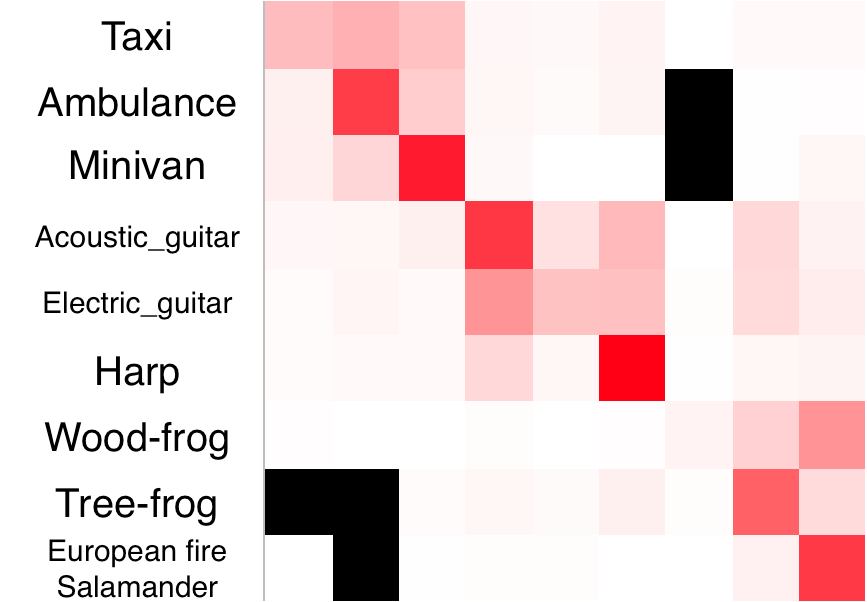
\includegraphics[width=1\textwidth ]{mc60}\caption{Matrice de confusion 60 itérations}
\end{minipage}
\begin{minipage}{.5\textwidth}
\centering

\includegraphics[width=0.55\textwidth]{mc600}\caption{Matrice de confusion 600 itérations}
\end{minipage}

\end{figure}

\noindent
 Nous remarquons que des zones rouges apparaissent au niveau des catégories mères (car, stringed\_instrument et amphibian) ceci signifie que les erreurs les plus fréquentes de classifications se font avec des catégories appartenant à la même classe mère. C'est un résultat normal étant donné qu'il est plus facile de confondre un taxi et une ambulance qu'un taxi et une salamandre par exemple. Par ailleurs nous pouvons remarquer que dans la matrice de confusion à 600 itérations il y a plus de cases noires (qui signifient qu'aucune erreur n'a été réalisé avec la classe en question) et que les zones rouges(zones de classification la plus fréquente) sont plus 'resserrées', cela veut dire que la classification est meilleure avec un classifieur apprit sur plus d'itérations. 
 
 Les images les plus difficiles à classifier sont les images de la catégorie wood-frog qui sont souvent confondues avec tree-frog ou salamander, les images de la catégorie taxi qui sont confondues avec ambulance et minivan et les images de la catégorie electric-guitar qui sont souvent classifiés comme acoustic-guitar et harp.

Les taux de bonne classification du classifieur multi-classes sont les suivants.\\
\begin{center}
\begin{tabular}{|c|c|}
\hline
 & Classifieur multi-classe \\
\hline
\hline
60 itérations & 0.5375\\
600itérations & 0.5810\\
\hline
\end{tabular}
\end{center}


\section*{4.Classifieur hiérarchique}
\addcontentsline{toc}{section}{4.Classifieur hiérarchique}
Le classifieur hiérarchique prend en compte l'ontologie de WordNet en effet la fonction $\Delta(y,y')$ qui représente la dissimilarité entre deux classe y et y' n'est plus le 0-1 loss mais la fonction $1-similarity(y,y')$ de WuPalmer. Ce changement de fonction de dissimilarité vise à ne pas trop impacter la fonction de cout lorsque l'erreur est faite avec une classe proche sémantiquement. 

\subsection*{1.Evaluation du classifieur hiérarchique}
\addcontentsline{toc}{subsection}{1.Evaluation du classifieur hiérarchique}
De la même manière que pour le classifieur multi-classes nous avons affiché la matrice de confusion pour évaluer l'erreur de classification et mieux comprendre avec quelles classes le classifieur a des difficultés. Là encore nous pouvons remarquer que plus il y a d'itérations (matrice de droite) plus les zones rouges sont recentrées sur les catégories de la même famille sémantique, c'est à dire que l'algorithme classifie mieux ou en tout cas fait des erreurs moins grave, c'est à dire qu'il se peut qu'il fasse des erreurs mais se sont des classifications erronées sur les mêmes catégorie mères. Nous pouvons aussi faire la comparaison avec les matrices de confusion du classifieur multi-classes puisque nous pouvons très bien voir que les zones d'erreur rouge sont bien plus centrées sur les classes ou l'erreur est moins préjudiciable pour ce qui est du classifieur hiérarchique. Voila pourquoi, pour ce genre de classification sur une structure hiérarchique il est important de prendre en compte la distance entre catégories pour classifier des éléments et non pas utilisé un 0-1 loss qui fait perdre cette information et résulte sur des classifications moins pertinentes.\\\\


\begin{figure}[H]
\centering

\begin{minipage}{.45\textwidth}
\centering
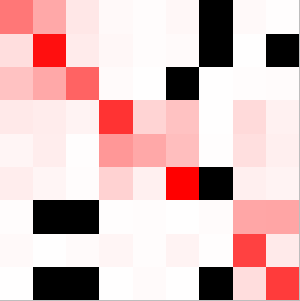
\includegraphics[width=0.5\textwidth ]{mc_60hier}\caption{Matrice de confusion \\60 itérations}
\end{minipage}
\begin{minipage}{.45\textwidth}
\centering

\includegraphics[width=0.5\textwidth]{mc_600hier}\caption{Matrice de confusion \\600 itérations}
\end{minipage}

\end{figure}

Les taux de bonne classification du classifieur hiérarchique sont les suivants.\\
\begin{center}
\begin{tabular}{|c|c|}
\hline
& Classifieur hiérarchique \\
\hline
\hline
60 itérations & 0.5378\\
600itérations & 0.5662\\
\hline
\end{tabular}
\end{center}


\section*{5.Comparaison entre le classifieur multi-classes et le hiérarchique}
\addcontentsline{toc}{section}{5.Comparaison entre le classifieur multi-classes et le hiérarchique}
Nous rappelons les taux de bonne classifications pour les deux classifieurs (multi-classes et multi-classes hiérarchique).\\
\begin{center}
\begin{tabular}{|c|c|c|}
\hline
&Classifieur multi-classes &  Classifieur hiérarchique \\
\hline
\hline
60 itérations & 0.5375 & 0.5378\\
600 itérations & 0.5810 & 0.5662\\
\hline
\end{tabular}
\end{center}
 Nous remarquons que pour un nombre d'itérations égale à 600 le classifieur multi-classes obtient de meilleurs performances (0.5810) que le classifieur hiérarchique (0.5662). Ces résultats sont différents puisque nous n'utilisons pas les mêmes calculs de dissimilarité entre classe dans la fonction de cout. Le classifieur multi-classes minimise le taux d'erreur général (sans prendre en compte les distances inter-classes entre catégories) alors que le classifieur hiérarchique préfère se tromper tant qu'il fait des erreurs inter-classes (il prend en compte les distances entre catégories). Voilà pourquoi le classifieur multi-classe obtient un meilleur taux de classification sur l'ensemble des tests.\\\\
En revanche lorsque nous calculons le taux de bonne classification non pas en fonction des classes mais en fonction des catégories mères. Par exemple si une image de salamander est catégorisée comme une tree-frog nous comptons cela comme une bonne classification comme elles font partie de la même catégorie mère (amphibian). Nous obtenons de meilleurs taux de bonne classification avec le classifieur hiérarchique.

\begin{center}
\begin{tabular}{|c|c|c|}
\hline
&Classifieur multi-classes &  Classifieur hiérarchique \\
\hline
\hline
Taux classif - classe mère & 0.7517 & 0.7624\\

\hline
\end{tabular}
\end{center}
\section*{6.Modèles de ranking}
\addcontentsline{toc}{section}{6.Modèles de ranking}
Le ranking consiste dans notre cas à renvoyer les images par ordre décroissant de score de similarité entre ces images de la base et une catégorie donnée. Pour une catégorie donnée (exemple charmander) nous voulons que toutes les images de test de la base correspondant au label 'charmander' soient renvoyées en premier, d'où le score de similarité plus important et le classement décroissant. 
\subsection*{1.Evaluation du ranking}
\addcontentsline{toc}{subsection}{1.Evaluation du ranking}
Nous avons utilisé deux mesures d'évaluation du résultat de ranking. La première est la courbe de précision rappel. Pour rappel:\\\\
$Rappel_i = \frac{documents~correctement~attribu\acute{e}s~\grave{a}~la~classe~i}{nombre~de~documents~appartenant~\grave{a}~la~classe~i} $\\\\
$Pr\acute{e}cision_i = \frac{documents~correctement~attribu\acute{e}s~\grave{a}~la~classe~i}{nombre~de~documents~attribu\acute{e}s~\grave{a}~la~classe~i} $\\\\

Nous obtenons ces différentes courbes de PR (précision-rappel):\\
\noindent
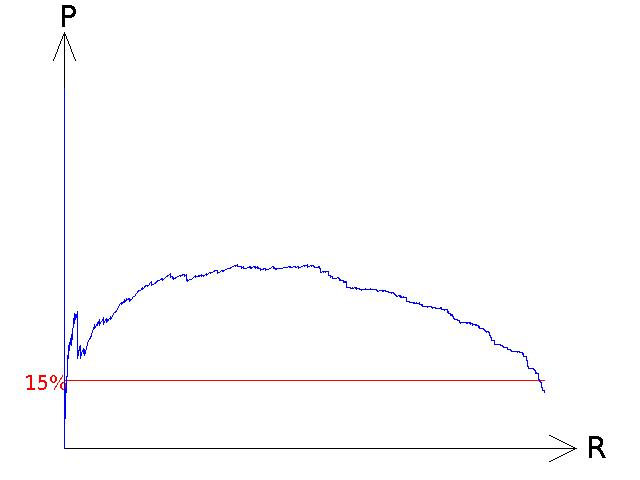
\includegraphics[width=0.3\textwidth]{RP_acoustic_guitar.jpg}\hfill
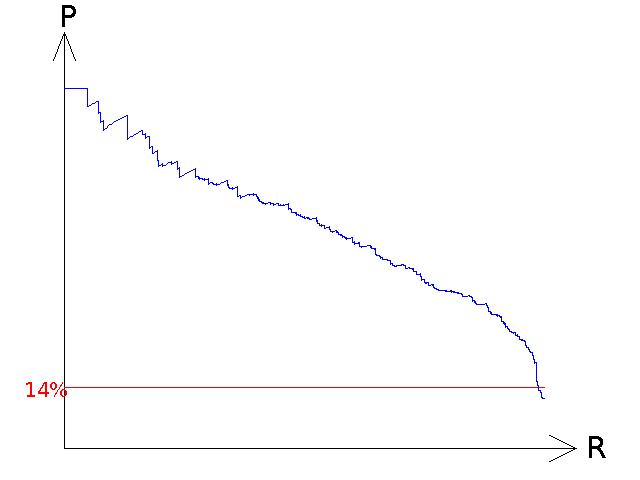
\includegraphics[width=0.3\textwidth]{RP_harp.jpg}\hfill
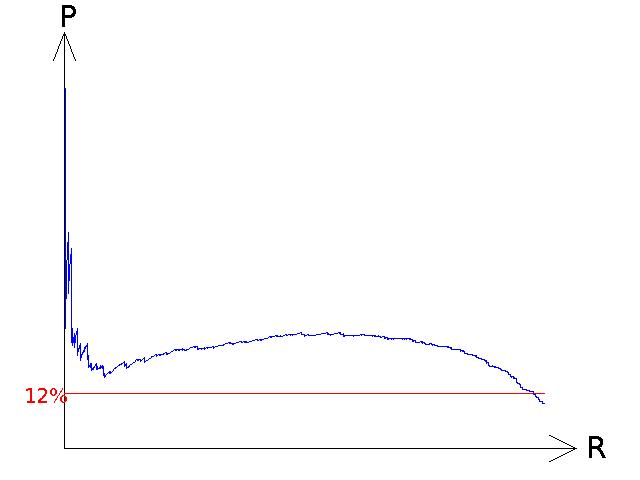
\includegraphics[width=0.3\textwidth]{RP_electric_guitar.jpg}\\
.~~~~~~~~~~~~~acoustic guitar ~~~~~~~~~~~~~~~~~~~~~~harp~~~~~~~~~~~~~~~~~~~~~~~~~~ electric guitar\\\\
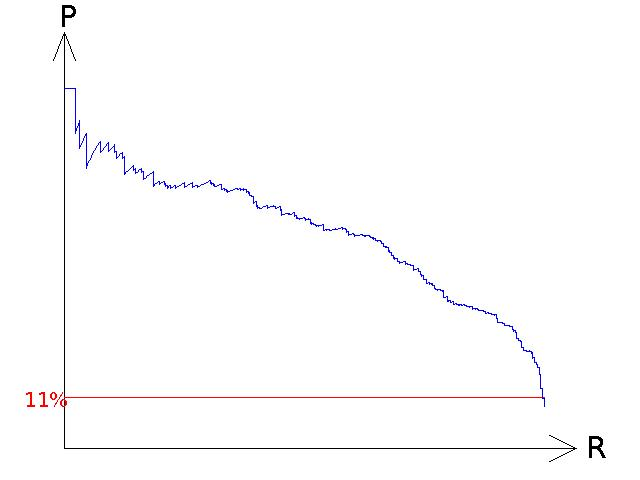
\includegraphics[width=0.3\textwidth]{RP_ambulance.jpg}\hfill
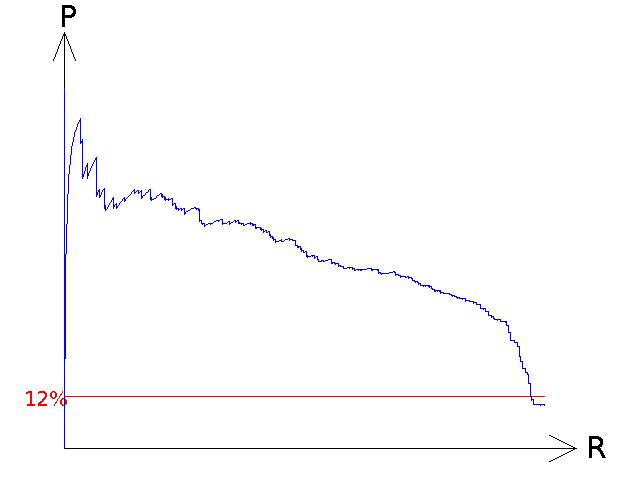
\includegraphics[width=0.3\textwidth]{RP_minivan.jpg}\hfill
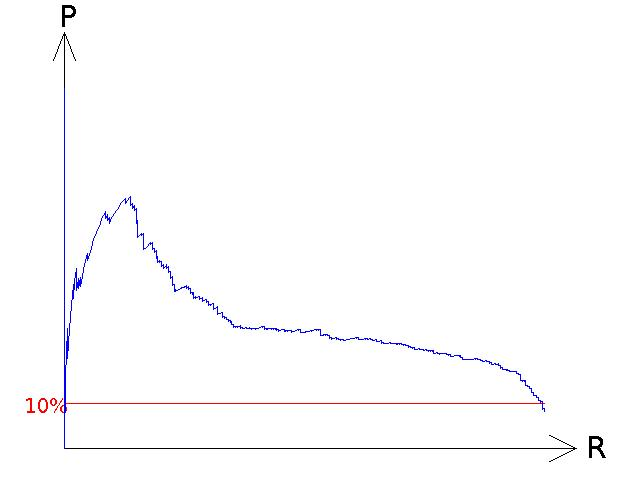
\includegraphics[width=0.3\textwidth]{RP_taxi.jpg}\\
.~~~~~~~~~~~~~ambulance ~~~~~~~~~~~~~~~~~~~~~~minivan~~~~~~~~~~~~~~~~~~~~~~~~~~ taxi\\
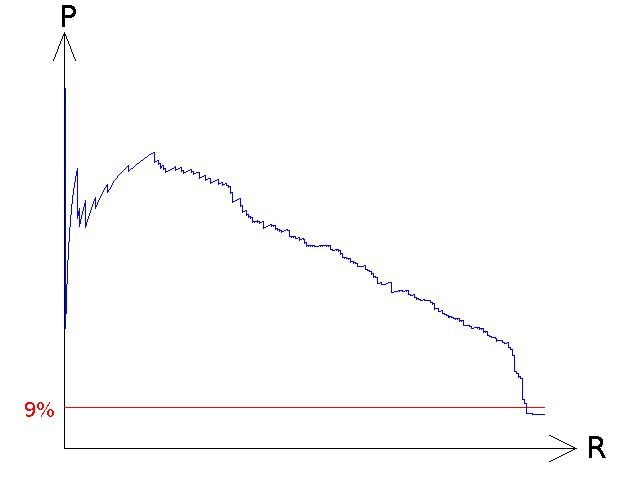
\includegraphics[width=0.3\textwidth]{RP_tree-frog.jpg}\hfill
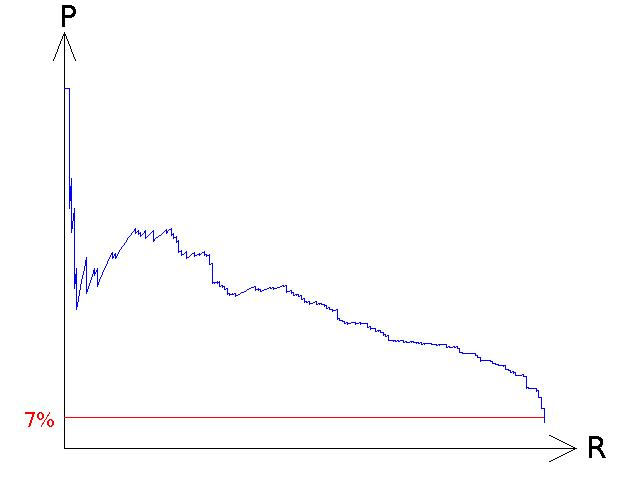
\includegraphics[width=0.3\textwidth]{RP_wood-frog.jpg}\hfill
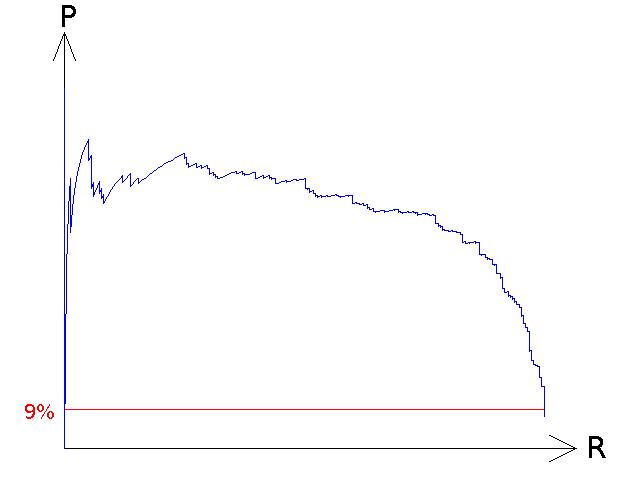
\includegraphics[width=0.3\textwidth]{RP_european_fire_salamander.jpg}\\
.~~~~~~~~~~~~~tree frog~~~~~~~~~~~~~~~~~~~~~~wood frog~~~~~~~~~~~~~~~~~~~~~~~~~~ european\_fire\_salamander\\\\

L'ensemble des courbes suivent le même shémas elle ont une forte précision pour peu d'élément rankés et la précision diminue avec plus d'éléments, ceci est normal puisque plus il y a d'élément à ranker plus la précision diminue puisque des erreurs adviennent.\\

La deuxième mesure d'évaluation est la mesure AP (average precision ou en français la précision moyenne). 
Nous obtenons ces résultat d'AP pour les classes Ambulance: , Wood-Frog: et Harp: .\\

\begin{center}
\begin{tabular}{|c|c|c|c|}
\hline
& ambulance & wood-frog & harp \\
\hline
\hline
AP & 0.6091 & 0.4026 & 0.6312 \\

\hline
\end{tabular}
\end{center}

Nous pouvons faire le parallèle avec la classification multi-classe en regardant les matrices de confusion. Nous remarquons clairement que la catégorie wood-frog qui a une AP de 0.40 (faible) est très mal classée par le classifieur multi-classes. En effet nous pouvons voir que dans la matrice de confusion la catégorie salamander est souvent prédite à la place de la catégorie wood-frog. En revanche pour la catégorie ambulance qui a une AP de 0.6091 (élevée) en ranking est mieux catégorisée par le classifieur multi-classes. Nous pouvons donc conclure que la précision moyenne (AP) obtenu en évaluant le ranking et les performances de classification obtenues par le classifieur multi-classes sont corrélées. 


\chapter*{Conclusion}
\addcontentsline{toc}{chapter}{Conclusion}
Lors de ce projet nous avons apprit à représenter les images sous forme vectoriel (BOW). Nous avons aussi créer des classifieurs de différents types, multi-classes et hiérarchique et évalué ces modèles de classifications. Pour finir nous avons crée un algorithme de ranking basé sur le score de classification des différentes images, pour ce modèle nous avons utilisé différentes méthodes d'évaluation. Pour aller plus loin il serait intéressant d'utiliser d'autres méthodes pour représenter les images telles que les CNN( convolutional neural network) permettant de représenter avec plus de précision une image sous forme de vecteur. Par ailleurs des techniques de localisation d'objet dans les images pourraient permettre de focaliser l'apprentissage sur la partie intéressante de l'image (là ou l'élément à classifier se situe) et ainsi éviter le bruit que peu apporter l'arrière plan de l'image. Pour cela nous pouvons imaginer utiliser des Spatial Transformer Networks permettant d'éliminer le bruit dès la classification d'image (qui serait faite entièrement avec un reseaux de neuronnes) et ainsi avoir une bonne représentation d'une image.


%\section*{1.Nom\_section}
%\addcontentsline{toc}{section}{1.Nom\_section}

%\subsection*{1.Nom\_subsection}
%\addcontentsline{toc}{subsection}{1.Nom\_subsection}

%\subsubsection*{1.Nom\_subsubsection}
%\addcontentsline{toc}{subsubsection}{1.Nom\_subsubsection}





%ajouter des images png \hfill si ajout d'une autre photo à côté
%\includegraphics[width=0.5\textwidth]{nom_image}\hfill
%\includegraphics[width=0.5\textwidth]{nom_image}



\end{document}
